% LTeX: enabled=true

\chapter{Commande hybride}
\label{chap:hybrid}
\minitoc


\section{Motivation}
En prenant en compte les capacités d'un \textit{tailsitter}, il est légitime de se poser la question du mode de vol devant être utilisé pour rejoindre un point. Effectivement, le drone a la possibilité de se déplacer en stationnaire ou bien en vol d'avancement. Lors d'un déplacement en stationnaire, le drone est vertical donc il se retrouve fortement sujet aux perturbations. Il est donc nécessaire d'avoir une grande région d'attraction autour de la position d'équilibre pour assurer un rejet des perturbations et une stabilisation. Lors d'un vol d'avancement, le drone se trouve dans une configuration proche d'une aile volante. Ainsi, il se trouve moins perturbé par les turbulences, dans la mesure où la surface projetée d'aile impactée par le flux d'air est plus faible. Toutefois, le drone doit voler à une vitesse assez importante pour être dans cette configuration donc il ne peut pas maintenir une position, mais seulement effectuer des cercles autour. 

Nous nous concentrons dans ce chapitre uniquement au vol stationnaire. Il s'agit donc de proposer une stratégie de commande pour stabiliser le drone en position stationnaire. Cette stratégie repose sur une dynamique discrète définissant l'usage d'une première loi de commande non-linéaire présentée dans \cite{2020e-MicCenZacFra} et qui fournit une grande région d'attraction et d'une seconde loi basée sur la dynamique linéarisée et fournissant une agressivité supérieure pour réaliser l'approche finale. Les deux contrôleurs sont réunis par un mécanisme hybride qui permet de conserver les performances en régime permanent de la conception linéarisée, avec la grande région d'attraction garantie par la conception non linéaire. Notre solution est testée en simulant le modèle non linéaire complet.

Dans cette partie, nous allons nous concentrer sur la stabilisation stationnaire du drone. Ainsi nous nous appuyons sur la dynamique simplifiée décrite dans la section \ref{sec:model_NL_simp}, avec la simplification $\boldsymbol{w} = 0$ qui permet d'obtenir la dynamique simplifiée sans vent \eqref{eq:withouwind}. 



\section{Contrôleur par retour d'état non-linéaire}
Nous illustrons dans cette section une loi de contrôle dynamique non linéaire inspirée du résultat de \cite{2020e-MicCenZacFra}. Pour que cette loi de contrôle non linéaire soit applicable, les matrices $\boldsymbol{F}$ et $\boldsymbol{M}$ mentionnées dans \eqref{eq:withouwind} doivent permettre de définir une direction dite de zéro moment $\boldsymbol{\bar u} \in \real^4$ garantissant
$|\boldsymbol{F}\boldsymbol{\bar u}| = 1$ et $\boldsymbol{M} \boldsymbol{\bar u}=0$, et la matrice inverse à droite $\boldsymbol{M}^r$ de $\boldsymbol{M}$ doit satisfaire $\boldsymbol{M} \boldsymbol{M}^r = \mathbb{I}_3$ et $\boldsymbol{F}\boldsymbol{M}^r=0$. 

Dans notre cas, nous constatons que la direction du moment zéro $\boldsymbol{\bar u} = \frac{\sqrt{2}}{2a_{\text{f}}}\smallmat{1&1&0&0}^\top$ satisfait les conditions, alors que le fait que $\rank(\boldsymbol{F}) = 2$ (donc que le noyau de $\boldsymbol{F}$ ($\ker \boldsymbol{F}$) soit de dimension 2) rend impossible l'obtention de la matrice inverse à droite $\boldsymbol{M}^r$ de $\boldsymbol{M}$, laquelle est entièrement contenue dans $\ker \boldsymbol{F}$.

Nous déterminons $\boldsymbol{M}^r$ en paramétrant (de manière conservatrice) les  pseudo-inverses à droite de $\boldsymbol{M}$ comme $\boldsymbol{M}^r := \boldsymbol{K}\boldsymbol{M}^\top ( \boldsymbol{M}\boldsymbol{K}\boldsymbol{M}^\top)^{-1}$, où la matrice $\boldsymbol{K} \in \real^{4\times 4}$ est symétrique et satisfait $\boldsymbol{M}\boldsymbol{K}\boldsymbol{M}^\top \geq \mathbb{I}_3$ (pour assurer l'inversibilité). Avec ce paramétrage, le but est de minimiser la norme de $\boldsymbol{F}\boldsymbol{M}^r = \boldsymbol{F} \boldsymbol{K}\boldsymbol{M}^\top ( \boldsymbol{M}\boldsymbol{K}\boldsymbol{M}^\top)^{-1}$, ce qui est bien obtenu en minimisant la norme de $\boldsymbol{F} \boldsymbol{K}\boldsymbol{M}^\top$, du fait que la contrainte sur $\boldsymbol{M}\boldsymbol{K}\boldsymbol{M}^\top \geq \mathbb{I}_3$ garantit que le facteur $( \boldsymbol{M}\boldsymbol{K}\boldsymbol{M}^\top)^{-1}$ ait une norme plus petite que 1.
En effectuant un complément de Schur, cette minimisation est obtenue en résolvant le programme semi-défini suivant :
\begin{align*}
&  \min_{\boldsymbol{K}, \kappa} \kappa, \; \mbox{subject to:}
\;  \boldsymbol{M} \boldsymbol{K} \boldsymbol{M}^\top\! \geq \!\mathbb{I}_3, \; 
  \begin{bmatrix}
  \kappa \mathbb{I}_3  &\! \boldsymbol{F} \boldsymbol{K} \boldsymbol{M}^\top \\ 
  \boldsymbol{M} \boldsymbol{K}^\top \boldsymbol{F}^\top &\! \kappa \mathbb{I}_3
  \end{bmatrix}\! \geq\! 0,
\end{align*}
lequel minimise $\kappa$ tout en assurant $\boldsymbol{F} \boldsymbol{K} \boldsymbol{M}^\top \boldsymbol{M} \boldsymbol{K}^\top \boldsymbol{F}^\top \leq \kappa^2 \mathbb{I}_3$.  En résolvant cette optimisation, on obtient, pour les matrices spécifiques considérées,
\begin{align*}
    \boldsymbol{K} \!=\! \smallmat{  0   &   -737   &    171   &   -171\\
      -737  &  0   &  -171  &     171\\
       171  &    -171    &   1583.5    &   -43.73\\
      -171  &     171    &   -43.73    &   1583.5}\!, \,
      \boldsymbol{M}^r \!=\! \smallmat{0     &          0   &   -3.19\\
                 0      &         0   &    3.19\\
               -4.51    &  -27.75    &   -1.48\\
                4.51    &  -27.75    &    1.48}
\end{align*}
conduisant à $\kappa = 39,7$. Avec cette sélection basée sur l'optimalité, la conception dynamique non linéaire de \cite{2020e-MicCenZacFra} peut être appliquée efficacement en obtenant des réponses qui sont presque impossibles à distinguer du cas entièrement découplé 
$\boldsymbol{F}\boldsymbol{M}^r=0$. Il convient de noter qu'une approche similaire, négligeant essentiellement les termes supplémentaires agissant sur la dynamique de translation, est également suggérée dans l'étude \cite{hamel_minhduc}. 
Sur la base du choix de $\boldsymbol{M}^r$ et de $\boldsymbol{\bar u}$ décrit ci-dessus, en appliquant la loi de commande de \cite[eqn (19)]{2020e-MicCenZacFra}, l'entrée $\boldsymbol{u}$ devient :
\begin{align}
\label{eq:u_nonlin}
    \boldsymbol{u} = \boldsymbol{u_{\text{nl}}} := \boldsymbol{M}^r \boldsymbol{\tau_{r}} + \boldsymbol{\bar u} \boldsymbol{f},
\end{align}
où $\boldsymbol{\tau_{r}}$ et $\boldsymbol{f}$ sont fournis par le contrôleur proposé dans \cite{2020e-MicCenZacFra}.


La sélection de $\boldsymbol{M}^r$ basée sur l'optimalité peut être interprétée de manière intéressante lorsqu'on observe le produit $\boldsymbol{M}^r \boldsymbol{\tau_{r}} = \boldsymbol{M}^r \smallmat{\tau_{r,x} & \tau_{r,y} & \tau_{r,z}}^top$. 

Premièrement, pour obtenir un moment $\tau_{r,z}$ autour de l'axe $z_{\text{b}}$, nous utilisons principalement l'action différentielle de la poussée ; deuxièmement, un moment $\tau_{r,y}$ autour de l'axe $y_{\text{b}}$ est généré par une utilisation symétrique des deux volets, avec une grande efficacité ; enfin, un moment $\tau_{r,x}$ autour de l'axe $x_{\text{b}}$ provient d'une utilisation différentielle des volets. 

Enfin, par rapport à la solution proposée dans \cite{2020e-MicCenZacFra}, pour prendre partiellement en compte les effets de saturation énoncés dans la section~\ref{sec:saturation}, le bouclage décrit dans \cite{2020e-MicCenZacFra} a été augmenté d'une stratégie de saturation d'erreur ne permettant jamais à l'erreur de position $\boldsymbol{\rm e}_p$ utilisée dans \cite[eqn. (22)]{2020e-MicCenZacFra} de dépasser la valeur maximale de 3 mètres. Les autres gains de réglage nécessaires à la solution de \cite{2020e-MicCenZacFra} ont été sélectionnés en suivant une procédure de réglage des gains proportionnels et dérivés, cela conduit à $k_{pp} = 0.5$, $k_{pd} = 1.2$, $k_{ap} = 0.08$, $k_{ad} = 0.1$ et $k_{\Delta} = 1$.
 
La figure~\ref{fig_global_contol} montre la réponse du système en termes de positions, d'orientations (deux lignes du haut) et d'efforts des actionneurs (deux lignes du bas) lorsque le système part de la condition initiale $\boldsymbol{x(0)} = [\boldsymbol{p(0)}~ \boldsymbol{v(0)}~ \boldsymbol{q(0)}~ \boldsymbol{\omega_b(0)}]^\top = [0~0~0 ~ 0~0~0 ~0. 9140 ~0.1134~ -0.3728~ 0. 1134~ 0~ 0~ 0]^\top $ avec une position d'équilibre cible de $\boldsymbol{p_{\text{eq}}} = [4~5~6]^\top$ et $\boldsymbol{q_{\text{eq}}} = [\frac{\sqrt{2}}{2}~0~-\frac{\sqrt{2}}{2}~0]^\top$. 
Une réponse adéquate peut être observée, laquelle reste assez éloignée des saturations des actionneurs (voir section~\ref{sec:saturation}). L'augmentation des gains peut accélérer la réponse, mais produit toutefois des oscillations d'attitude indésirables. Il est donc intéressant de combiner ce contrôleur non linéaire (qui fournit une grande région d'attraction) avec un contrôleur plus agressif, conçu sur la base de la dynamique linéarisée sans vent \eqref{eq:linearized}.


\begin{figure}[ht!]
    \centering
    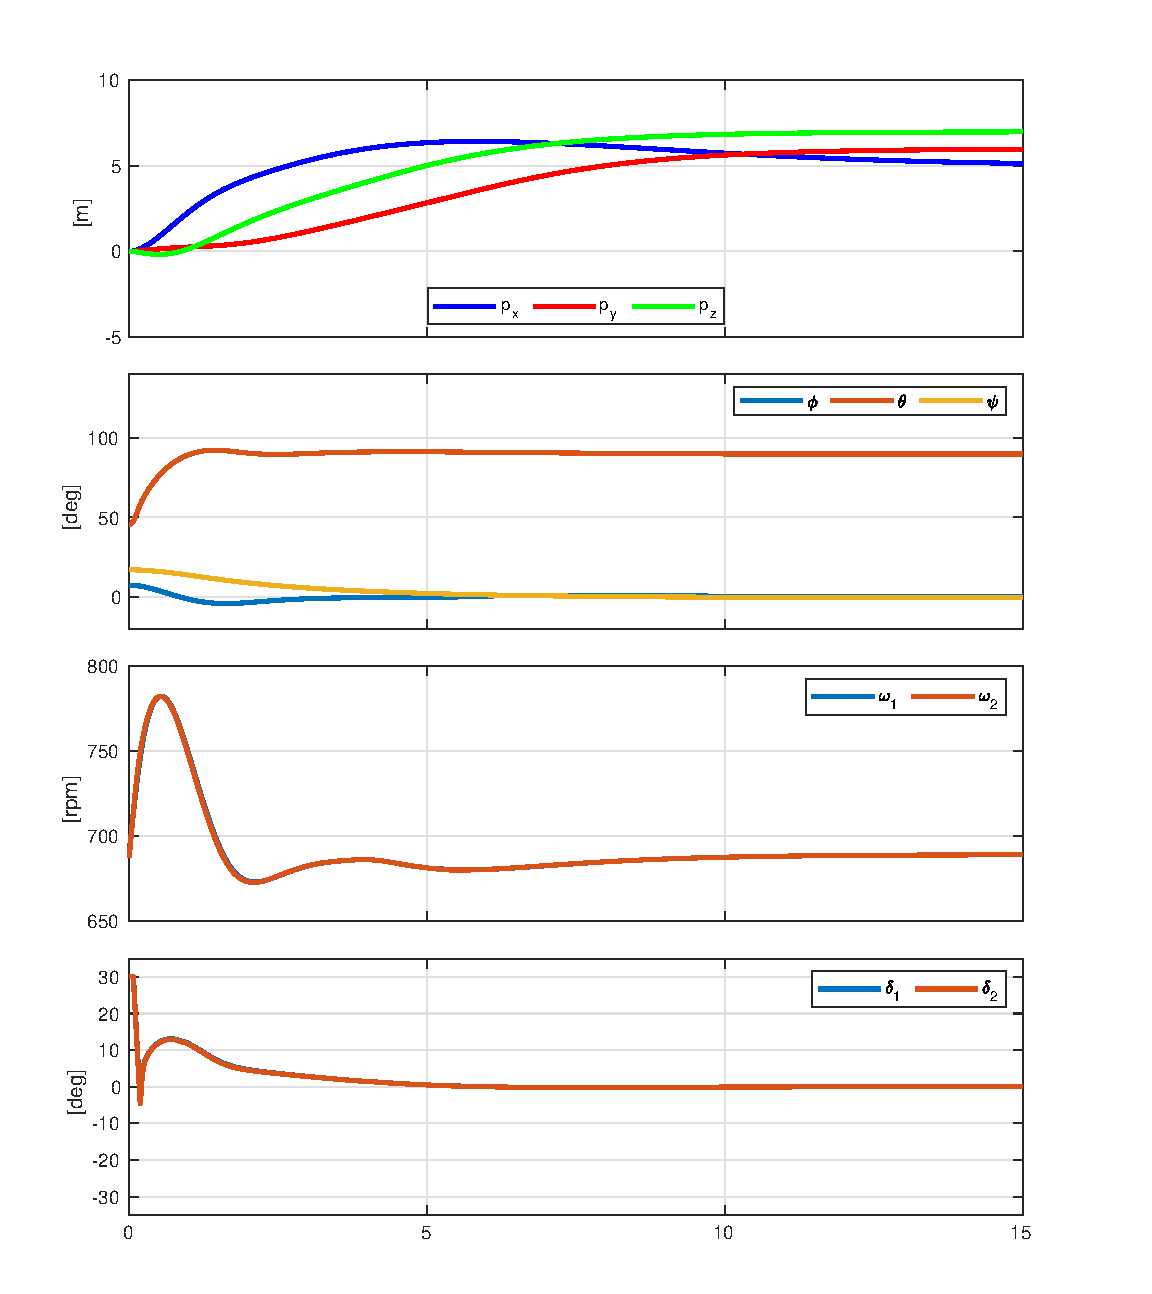
\includegraphics[trim=0cm 0.6cm 0cm 0.6cm,clip,width=0.8\columnwidth]{figures/global2.eps}
    \caption{Simulation de la loi de commande non-linéaire avec la dynamique de DarkO \eqref{eq:dyna_orig}.}
    \label{fig_global_contol}
\end{figure}


\section{Contrôleur par retour d'état linéaire}
Sur la base des observations de la section précédente et étant donné une position cible correspondant à un équilibre $\boldsymbol{p_{\text{eq}}}, \boldsymbol{q_{\text{eq}}}$ tel que caractérisé dans l'équation~\ref{eq:equilibria}, nous concevons ici un contrôleur par retour d'état linéaire capable de produire une réponse plus agressive. Pour cela, nous nous concentrons sur la dynamique linéarisée \eqref{eq:linearized} et proposons une loi de commande de la forme :
\begin{align}
  \boldsymbol{u_{\text{lin}}} := \boldsymbol{u_{\text{eq}}} - \boldsymbol{K} \boldsymbol{\tilde x},
\label{eq:u_lin}
\end{align}
où $\boldsymbol{\tilde x}$ a été introduit dans \eqref{eq:linearized} et $\boldsymbol{K} \in \real^{4 \times 12}$ est un gain de retour d'état qui peut être sélectionné, sur la base des matrices $\boldsymbol{A}_{0}$ et $\boldsymbol{G}_{0}$ apparaissant dans \eqref{eq:linearized}, de telle sorte que la boucle fermée du retour d'état $A_{\text{cl}}:=\boldsymbol{A}_{0}-\boldsymbol{G}_{0}\boldsymbol{K}$ soit exponentiellement stable. 

Dans notre cas, nous avons utilisé une sélection basée sur la commande linéaire quadratique, LQR \nomenclature[]{\(LQR\)}{Commande linéaire quadratique (\textit{Linear Quadratic Regulators})}, associée aux matrices de pondération $\boldsymbol{Q} = I_{12}$ et $\boldsymbol{R} = I_{4}$, qui donne une réponse en boucle fermée désirable. La conception LQR fournit également une matrice définie positive  $\boldsymbol{S} \in \real^{12 \times 12}$ (solution de l'équation algébrique de Riccati) garantissant que $\boldsymbol{A}_{\text{cl}}^\top \boldsymbol{S} + \boldsymbol{S} A_{text{cl}} <0$. Il est donc possible d'utiliser $\boldsymbol{S}$ pour former une fonction de Lyapunov.  En particulier, il est bien connu, d'après le théorème d'approximation linéaire, que la fonction $V(\boldsymbol{\tilde x}) = \boldsymbol{\tilde x}^\top S \boldsymbol{\tilde x}$ est également une fonction de Lyapunov certifiant la stabilité exponentielle locale de $\boldsymbol{x_{\text{eq}}}$ pour la dynamique non-linéaire. Plus précisément, il existe un scalaire positif $\bar v \in \real$ tel que, le long de la dynamique \eqref{eq:dyna_orig}, nous avons :
\begin{align}
\label{eq:Vdecrease}
  V(\boldsymbol{\tilde x}) \leq \bar v \quad \Rightarrow \quad \dot V(\boldsymbol{\tilde x}) := \langle 
\nabla V(\boldsymbol{\tilde x}), \boldsymbol{\dot{\tilde x}}\rangle <0,
\end{align}
pour tout $\boldsymbol{\tilde x} \neq 0$ ; en d'autres termes, le sous-ensemble de $V(\boldsymbol{\tilde x}) \leq \bar v$ est contenu dans le bassin d'attraction de l'équilibre $\boldsymbol{x_{\text{eq}}}$.

La détermination du plus grand scalaire $\bar v$ assurant \eqref{eq:Vdecrease} est un problème complexe et des bornes inférieures conservatrices peuvent être déterminées en quantifiant l'effet des non-linéarités sur la dynamique. Puisque $\boldsymbol{\dot{\tilde x}}$ est une fonction de $\boldsymbol{x}$, il est assez facile d'évaluer algébriquement $\dot V(\boldsymbol{\tilde x})$ pour un grand nombre d'extractions aléatoires de la variable $\boldsymbol{\tilde x}$, afin d'obtenir une estimation probabiliste du plus grand scalaire $\bar v$. Des garanties rigoureuses sur ces sélections peuvent être obtenues en appliquant les résultats de \cite{tempo2013randomized}, mais une évaluation de 10000 échantillons a confirmé que la valeur $\bar v = 400$ est une sélection satisfaisant \eqref{eq:Vdecrease}.


\begin{figure}[ht!]
    \centering
    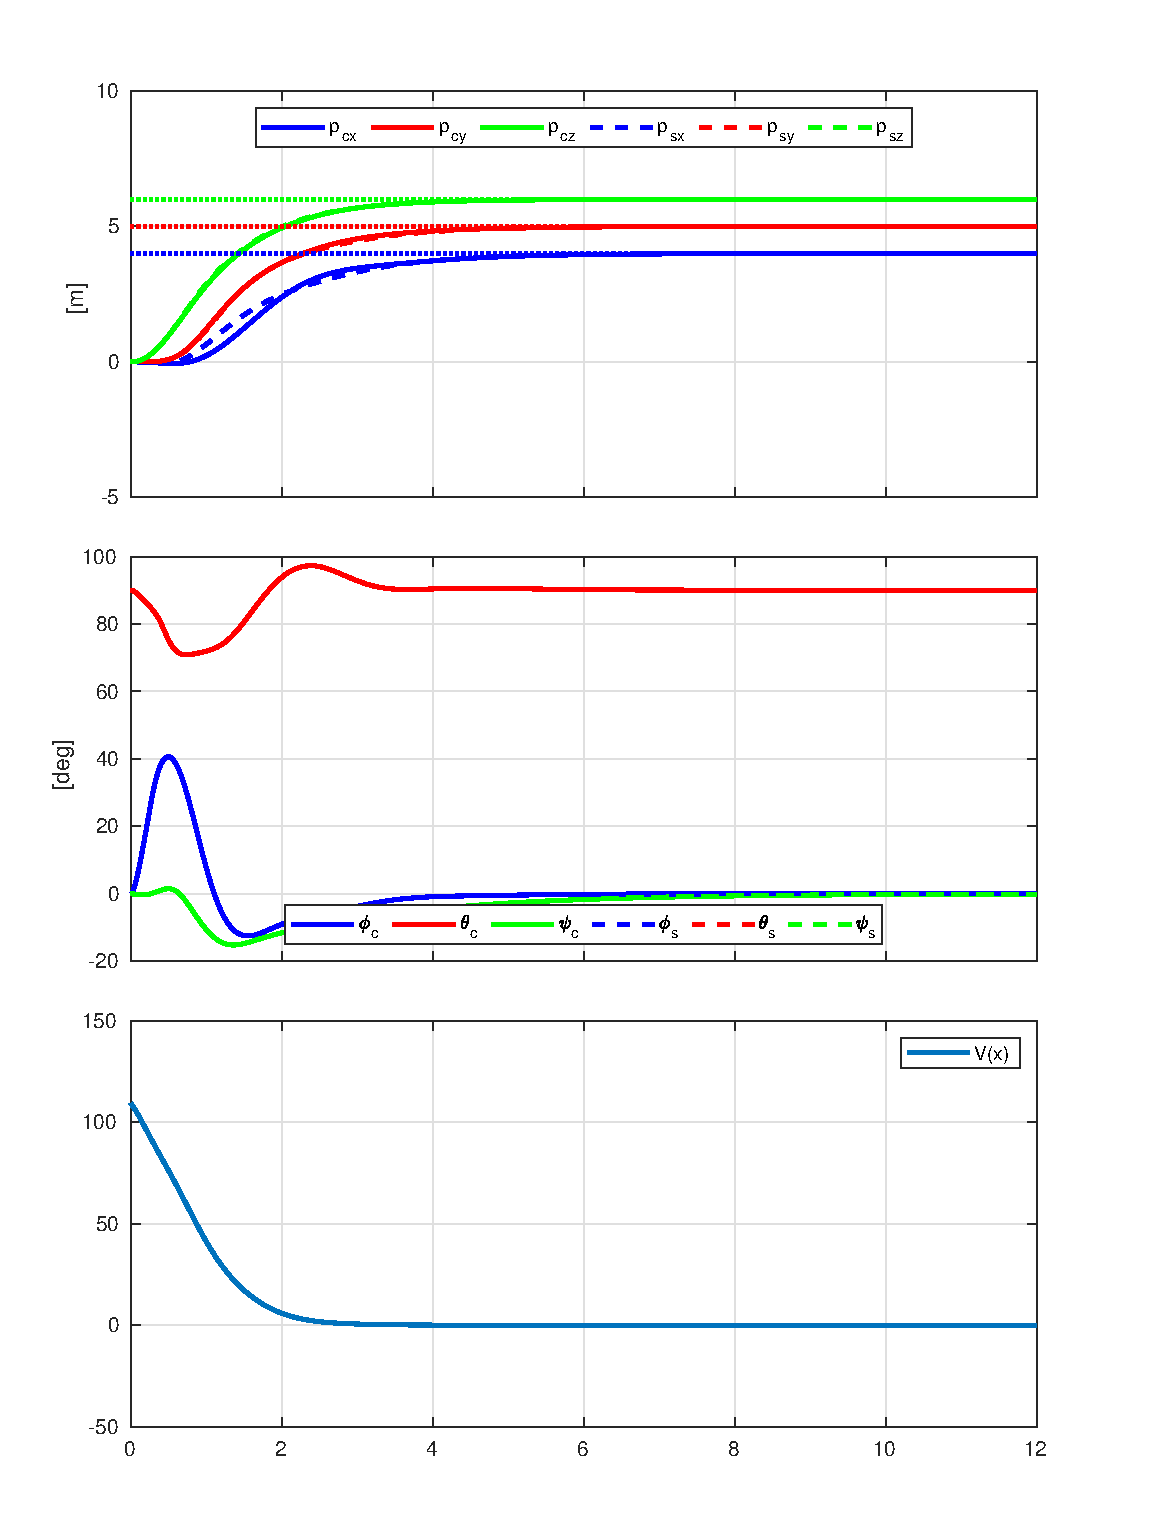
\includegraphics[trim=0cm 0.6cm 0cm 1cm,clip,width=0.8\columnwidth]{figures/converge2.eps}
    \caption{Simulation du modèle complet \eqref{eq:dyna_orig} (ligne continue) et simplifié \eqref{eq:withouwind} (ligne en pointillé) avec $\boldsymbol{u} = \boldsymbol{u}_{\text{lin}}$ défini dans 
    \eqref{eq:u_lin} et comme condition initiale $\tilde{ \boldsymbol{x}}_0$ dans le bassin d'attraction.}
    \label{fig_linearize_conv}
\end{figure}

La figure \ref{fig_linearize_conv} montre une simulation commençant à l'origine avec un drone vertical et des vitesses linéaires et angulaires initiales sont nulles. La position cible est $\boldsymbol{p_{\text{eq}}} = [4,~5,~6]$ avec une stabilisation en vol stationnaire (drone vertical) avec $\beta = 0$. La ligne en pointillé représente la position de la cible sur chaque axe. Le dernier graphique montre la décroissance exponentielle souhaitable de $V$.
La figure \ref{fig_linearize_conv} montre, à la fois, la simulation du modèle complet (continue) \eqref{eq:dyna_orig} et du modèle non linéaire simplifié \eqref{eq:withouwind} (en pointillé), ce qui met en évidence des différences dans la phase transitoire.
Lorsqu'on fournit une position cible plus importante $\boldsymbol{p_{\text{eq}}} =[8,~9,~10]$(avec la même orientation), la condition initiale se situe en dehors du bassin d'attraction et une divergence apparaît, comme le montre la figure~\ref{fig_linearize_div}.

\begin{figure}[ht!]
    \centering
    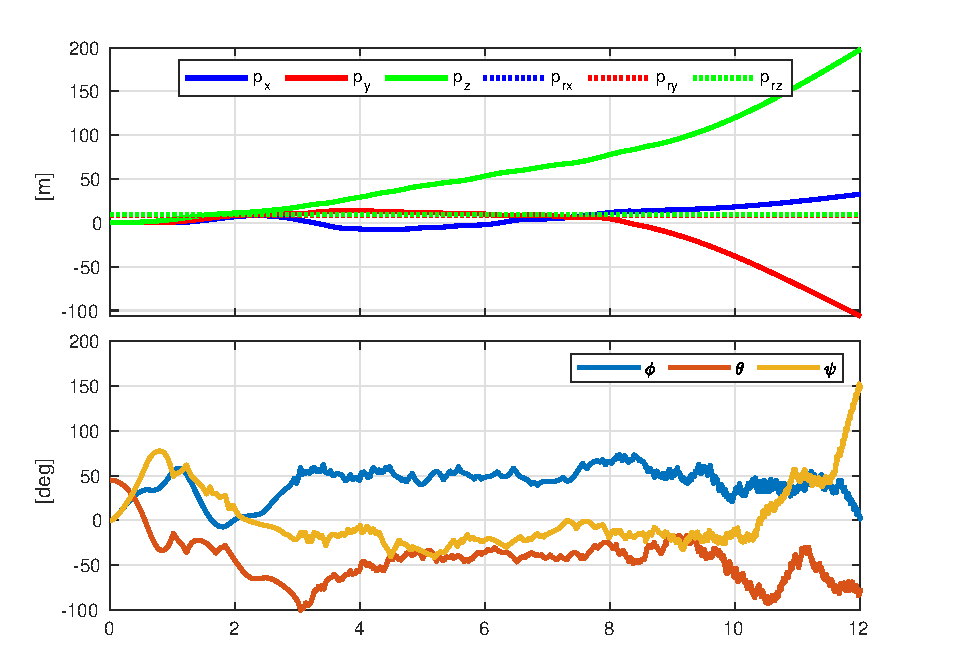
\includegraphics[trim=0cm 0cm 0cm 0cm,clip,width=0.8\columnwidth]{figures/diverge2.eps}
    \caption{Simulation divergente du modèle complet \eqref{eq:dyna_orig} avec $\boldsymbol{u} = \boldsymbol{u}_{\text{lin}}$ défini dans 
    \eqref{eq:u_lin} et une condition initiale $\tilde{ \boldsymbol{x}}_0$ en dehors du bassin d'attraction.}
    \label{fig_linearize_div}
\end{figure}



\section{Conception d'une commande locale-globale }
\label{sec:ctrl_hyste}
 
Considérant les stratégies locales-globales présentées dans \cite[Ex. 1. 7]{65}, similaires à la solution présentée dans \cite{AndreettoFZ16}, nous utilisons un mécanisme hybride sélectionnant le contrôleur local agressif \eqref{eq:u_lin} (tant que l'état se trouve dans le bassin d'attraction de l'équilibre) ou le contrôleur non linéaire moins agressif \eqref{eq:u_nonlin}, qui fournit une plus grande région d'attraction (et peut être appelé, par abus de langage, le "contrôleur global"). À cette fin, nous ajoutons à l'état du contrôleur une variable d'état logique $\ell \in \{0,1\}$, qui régit le choix de l'entrée de contrôle entre \eqref{eq:u_nonlin} et \eqref{eq:u_lin} tel que :
\begin{align}
\label{eq:u_hybrid}
  \boldsymbol{u}=\boldsymbol{u}_{\text{hyb}} := \ell \boldsymbol{u}_{\text{nl}} + (1-\ell) \boldsymbol{u}_{\text{lin}}.
\end{align}
Nous nous assurons, grâce à la dynamique hybride, que $\ell$ ne puisse prendre que des valeurs dans $\{0,1\}$. Sa dynamique est définie par : 
\begin{align*}
    \left\{
        \begin{array}{ll}
            \dot \ell = 0,& \chi \in \mathcal{C}\\
            \ell^{+} = 1-\ell,& \chi \in \mathcal{D}
        \end{array}
    \right.
\end{align*}
où $\chi = \left[\boldsymbol{p},~ \boldsymbol{v},~ \boldsymbol{q},~  \boldsymbol{\omega},~ l\right]$ est l'état complet de la boucle fermée et $\mathcal{C}$ et $\mathcal{D}$ sont, respectivement, les ensembles continus et discrets, définis par :
\begin{align*}
    & \mathcal{C} := \mathcal{C}_{0} \cup \mathcal{C}_{1}, ~ \mathcal{D} := \mathcal{D}_{0} \cup \mathcal{D}_{1},\\
   & \mathcal{C}_{0} :=\{\boldsymbol{\chi} \in \mathbb{R}^{14}:~ V(\boldsymbol{\tilde x}) \le \overline{v} \mbox{ and } \ell=0\}\\
   & \mathcal{C}_{1} :=\left\{\boldsymbol{\chi} \in \mathbb{R}^{14}:~ V(\boldsymbol{\tilde x}) \ge \underline{v} \mbox{ and } \ell=1 \right\}\\
   & \mathcal{D}_{0} :=\left\{\boldsymbol{\chi} \in \mathbb{R}^{14}:~ V(\boldsymbol{\tilde x}) \geq \overline{v}\mbox{ and } \ell=0 \right\}\\
   & \mathcal{D}_{1} :=\left\{\boldsymbol{\chi} \in \mathbb{R}^{14}:~ V(\boldsymbol{\tilde x}) \leq \underline{v}\mbox{ and } \ell=1 \right\}
\end{align*}
où $V(\boldsymbol{\tilde x}) := \boldsymbol{\tilde x}^\top S \boldsymbol{\tilde x}$  a été défini dans la section précédente, $\overline{v}=400$ a été déterminée pour satisfaire \eqref{eq:Vdecrease} et $\underline{v}$ est toute constante positive satisfaisant $\underline{v}<\overline{v}$ (un choix plus grand de $\underline{v}$ augmente la marge d'hystérésis, mais retarde le changement de loi de commande). Dans notre cas, nous choisissons $\underline{v}= 350$.

Le résultat suivant est une conséquence immédiate des résultats de \cite[Ex. 1.7]{65} et des propriétés de nos modèles linéaires et non linéaires.

\begin{proposition}
    Avec l'action du bouclage hybride \eqref{eq:u_hybrid}, la boucle fermée présente, quand elle utilise le contrôleur linéaire \eqref{eq:u_lin}, le même bassin d'attraction que celui associé au contrôleur non linéaire \eqref{eq:u_nonlin}.
\end{proposition}

Nous avons réalisé plusieurs simulations de la boucle fermée à l'aide de la \textit{toolbox} Matlab \cite{sanfelice_2017}. Les simulations sont effectuées avec le modèle complet du drone \eqref{eq:dyna_orig}, comprenant tous les effets aérodynamiques non linéaires. Un exemple de simulation est présenté dans la Figure~\ref{fig_sim}, où nous initialisons le drone à l'origine avec une orientation nulle, sauf pour l'angle de tangage fixé à 45 degrés. L'orientation de la cible est en configuration de vol stationnaire vertical et la position de la cible est assignée à $\boldsymbol{p_{\text{eq}}} = [50,~25,~12.5]$.

\begin{figure}[!ht]
    \centering
    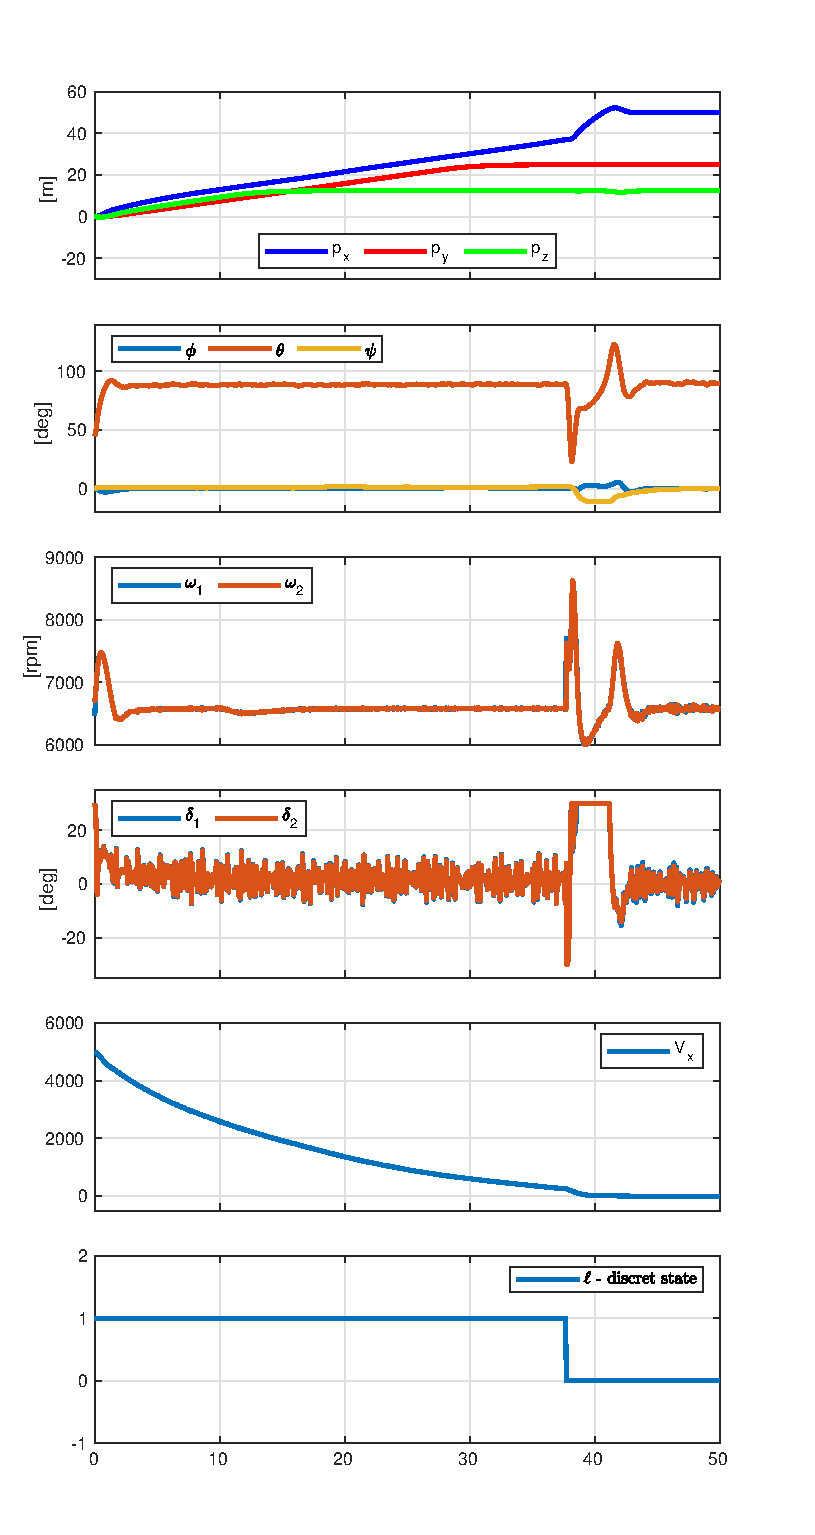
\includegraphics[trim=0cm 0cm 0cm 1.1cm,clip,width=0.8\columnwidth]{figures/switch_paper2.eps}
    \caption{Simulation en boucle fermée avec le contrôleur hybride \eqref{eq:u_hybrid}.}
    \label{fig_sim}
\end{figure}

Nous observons que sur la période $t \in \left[0,38\right]$, le drone
présente une convergence élégante mais lente vers la position cible souhaitée, en utilisant le contrôleur global ($\ell=1$). Dès lors, l'état discret $\ell$ entre dans l'ensemble $\mathcal{D}_1$ et le contrôleur local plus agressif est activé jusqu'à la convergence vers l'équilibre souhaité.

Pour obtenir des simulations réalistes, les mesures sont affectées par 
le bruit des capteurs. La robustesse intrinsèque de la rétroaction hybride, établie dans \cite[Chapitre 7]{65}, est confirmée par le maintien des performances, malgré le bruit de mesure.

\section{Conclusion du Chapitre \ref{chap:hybrid}}

{\color{red}
L'objectif principal de ce chapitre est de proposer un mécanisme hybride capable d'utiliser deux modes de contrôle d'un drone convertible, pour naviguer entre deux points. 

À partir du modèle simplifier proposé dans le chapitre \ref{chap:model}, nous avons proposé deux lois de contrôle, basées sur une linéarisation du modèle et sur un contrôle non linéaire.
Pour le vol stationnaire, nous avons utilisé une linéarisation autour d'un point d'équilibre sans vent, afin d'obtenir une loi de commande linéaire par retour d'état. L'avantage de cette dernière réside dans sa capacité à optimiser le retour d'état et donc à ajuster sa vitesse de convergence et à rejeter des perturbations.  Cependant, son domaine de stabilité est réduit, car il s'agit d'une loi de commande locale, valable dans le voisinage du point d'équilibre. Au contraire, la seconde loi proposée, non linéaire, est globale. Celle-ci, stable sur l'ensemble du domaine de vol, ne permet cependant pas d'optimiser la vitesse de convergence, compte tenu de sa complexité.

Compte tenu des avantages et des inconvénients observés dans les lois de commande, il a semblé approprié d'envisager une transition hybride sur la base de la stabilité de la boucle. En d'autres termes, le contrôleur non linéaire est utilisé là où le contrôleur linéaire est instable, afin de faire converger le drone vers la cible. Dès que le drone entre dans le domaine de stabilité du contrôleur linéaire, le mécanisme hybride prend en charge le changement de loi, en utilisant la vitesse de convergence maximale autorisée par l'optimisation linéaire. L'avantage de ce mécanisme est qu'il fournit un contrôleur ayant autorité sur l'ensemble du domaine de vol, assurant la convergence, tout en optimisant les capacités du drone. Bien que les premiers résultats ne soient obtenus que par simulation, ils semblent prometteurs pour une intégration sur l'architecture réelle.

Toutefois, ce travail ne prend pas en compte l'impact des turbulences ou du vent sur l'architecture \textit{tailsitter}. Il est donc intéressant de se focalisé sur des mécanismes de stabilisation d'un drone face à des conditions de vol plus réaliste.

}
